%%%%%%%%%%%%%%%%%%%%%%%%%%%%%%%%%%%%%%%%%
% a0poster Landscape Poster
% LaTeX Template
% Version 1.0 (22/06/13)
%
% The a0poster class was created by:
% Gerlinde Kettl and Matthias Weiser (tex@kettl.de)
% 
% This template has been downloaded from:
% http://www.LaTeXTemplates.com
%
% License:
% CC BY-NC-SA 3.0 (http://creativecommons.org/licenses/by-nc-sa/3.0/)
%
%%%%%%%%%%%%%%%%%%%%%%%%%%%%%%%%%%%%%%%%%

%----------------------------------------------------------------------------------------
%	PACKAGES AND OTHER DOCUMENT CONFIGURATIONS
%----------------------------------------------------------------------------------------

\documentclass[a0,landscape]{a0poster}

\usepackage{multicol} % This is so we can have multiple columns of text side-by-side
\columnsep=80pt % This is the amount of white space between the columns in the poster
\columnseprule=3pt % This is the thickness of the black line between the columns in the poster

\usepackage[svgnames]{xcolor} % Specify colors by their 'svgnames', for a full list of all colors available see here: http://www.latextemplates.com/svgnames-colors

\usepackage{times} % Use the times font
%\usepackage{palatino} % Uncomment to use the Palatino font

\usepackage{graphicx} % Required for including images
\graphicspath{{figures/}} % Location of the graphics files
\usepackage{booktabs} % Top and bottom rules for table
\usepackage[font=small,labelfont=bf]{caption} % Required for specifying captions to tables and figures
\usepackage{amsfonts, amsmath, amsthm, amssymb} % For math fonts, symbols and environments
\usepackage{wrapfig} % Allows wrapping text around tables and figures
\usepackage{tgbonum}
\usepackage{xcolor, colortbl}
\usepackage{multirow}

% Set costum color
\definecolor{lightgreen}{HTML}{D5E8D4}
\definecolor{lightblue}{HTML}{DAE8FC}
\definecolor{lightgrey}{HTML}{CECECE}

\setlength\parindent{0pt}

\begin{document}
	\fontfamily{cmss}\selectfont

%----------------------------------------------------------------------------------------
%	POSTER HEADER 
%----------------------------------------------------------------------------------------

% The header is divided into three boxes:
% The first is 55% wide and houses the title, subtitle, names and university/organization
% The second is 25% wide and houses contact information
% The third is 19% wide and houses a logo for your university/organization or a photo of you
% The widths of these boxes can be easily edited to accommodate your content as you see fit

\begin{minipage}[b]{0.20\linewidth}
	\centering
\includegraphics[width=15cm]{Bilder/logo_UniStuttgart.jpg} % Logo or a photo of you, adjust its dimensions here
\end{minipage}
%
\begin{minipage}[b]{0.60\linewidth}
	\veryHuge \centering\color{DodgerBlue} \textbf{Dialog Act Classification}\\ % Title
	\Huge\textit{using Word Embeddings \& Acoustic Features} \color{Black}\\[1cm] % Subtitle
	\huge \textbf{Jens Beck, Fabian Fey, Richard Kollotzek}\\ % Author(s)
	\huge Institute for Natural Language Processing, University of Stuttgart\\ % University/organization
\end{minipage}
%
\begin{minipage}[b]{0.20\linewidth}
	\centering
\includegraphics[width=15cm]{Bilder/logo_IMS_klein.jpg} % Logo or a photo of you, adjust its dimensions here
\end{minipage}

\vspace{1cm} % A bit of extra whitespace between the header and poster content

%----------------------------------------------------------------------------------------

\begin{multicols}{3} % This is how many columns your poster will be broken into, a poster with many figures may benefit from less columns whereas a text-heavy poster benefits from more
%----------------------------------------------------------------------------------------
%	INTRODUCTION
%----------------------------------------------------------------------------------------

\color{Black} % SaddleBrown color for the introduction

\section*{Task Introduction}

%Dialog act classification is the task to label utterances with a category of meaning. For example to recognize whether the utterance is a question. In this poster we present an approach using a Convolution Neural Network (CNN) to classify utterances in four different classes (statement, question, opinion, backchannel). We depict an architecture with two different inputs. The Lexical model and the acoustic model. The lexical model works with the pretrained word2vec model provided by Google and the acoustic model works with MFCC features we extracted with openSmile. We put the two models together and gain a slightly better performance. 

\begin{itemize}
	\large
	\item Dialog Act Classification describes the process of automatically predicting the dialog act
	of the current speech and textual information
	\item We present an approach using a Convolutional Neural Network (CNN) which classifies utterances in four classes:
	\begin{itemize}
		\item statement (''I think I read about that in the paper'')
		\item question (''Well where do you take those things'')
		\item opinion (''It was really good'')
		\item backchannel (''Uh-huh'')
	\end{itemize}
	\item Two kinds of features:
	\begin{itemize}
		\item Lexical features
		\item Acoustic features 
	\end{itemize}
\end{itemize}
%- Dialog Act Classification\\
%- What are Dialog Acts\\
%-- Short examples\\

%----------------------------------------------------------------------------------------
%	MATERIALS AND METHODS
%----------------------------------------------------------------------------------------

\color{Black} % DarkSlateGray color for the rest of the content
\large

\section*{Data}
\subsection*{Switchboard}

\begin{itemize}
	\item We use a subset of the Switchboard Telephone Speech Corpus which consists of lexical and acoustic data
	\item Our subset includes 40,556 sentences
	\item The lexical dataset is divided in training, development and test data
	\item The acoustic dataset includes a recording for every utterance
\end{itemize}

\begin{tabular}{ l| c c c c || r}
	Dataset\textbackslash Channel & opinion & question & backchannel & statement & Sum\\
	\hline
	training & 4984 & 2150 & 6792 & 14459 & 28385\\
	development & 1068 & 460 & 1455 & 3098 & 6081\\
	test & 1070 & 463 & 1458 & 3099 & 6090\\
\end{tabular}

\subsection*{MFCC features}
\begin{itemize}
	\item With OpenSmile we extract the MFCC features for every sentence
	\item The MFCC features are extracted every 10ms with a frame size of 25ms
	\item This results in 13 features for each measurement point
\end{itemize}

\subsection*{word2vec}
\begin{itemize}
	\item For the word embedding layer we use the pre-trained Google word2vector model
	\item Contains 3 million words representing one word as a 300-dimensional vector
\end{itemize}

\large
\section*{Data Preprocessing}
\colorbox{lightblue}{
	\parbox{1025pt}{
		\vspace{0.5cm}
		{\LARGE \textbf{Embedding Matrix}}
		\begin{enumerate}
			\item All words from the training set are inserted into an embedding matrix
			\item Each word is represented by it's corresponding vector from \textit{word2vec}
			\item If a word is not contained in \textit{word2vec} it gets assigned a random vector
			\item Unkown word and no word vectors added
		\end{enumerate}
		\vspace{0.5cm}
		{\LARGE \textbf{Lexical Features}}
		\begin{enumerate}	
			\item Each sentence is converted into a sequence of indexes
			\item Each index is the corresponding line in the embedding matrix for one word
			\item The maximum sentence length is set to 100 words
		\end{enumerate}
}}
\colorbox{lightgreen}{
	\parbox{1025pt}{
		\vspace{0.5cm}
		{\LARGE \textbf{Acoustic Features}}
		\begin{enumerate}
			\item The MFCC features of the first 10 second are used
			\item The MFCC feature of the last 10 second are used 
			\item If audio file is shorter than 20 seconds the missing MFCC features are zeroized
		\end{enumerate}
	}}

%- Explanation of lexical and acoustic input\\
%-- Why 2000 MFCC-features\\
%----------------------------------------------------------------------------------------
%	RESULTS 
%----------------------------------------------------------------------------------------

\section*{System Architecture}
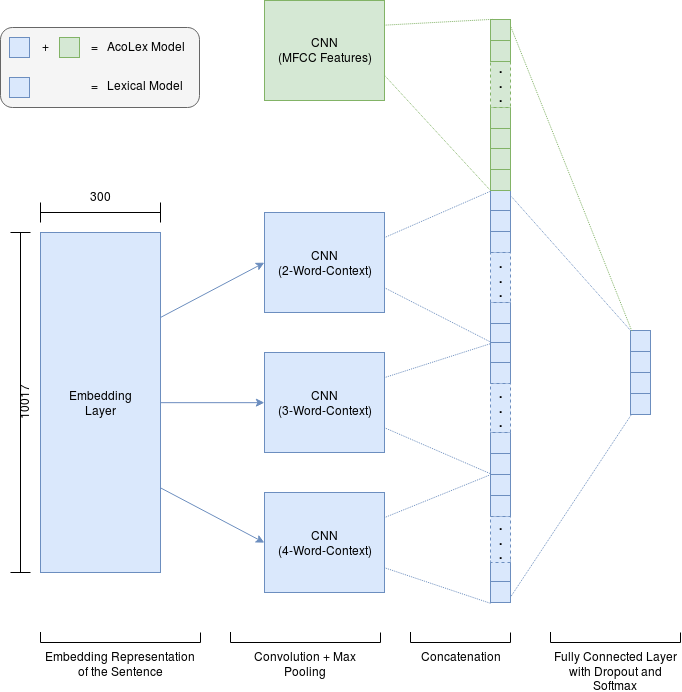
\includegraphics[width=0.9\linewidth]{Bilder/CNN_Diagram.png}

%----------------------------------------------------------------------------------------
%	CONCLUSIONS
%----------------------------------------------------------------------------------------

\color{Black} % SaddleBrown color for the conclusions to make them stand out
\large

\section*{Intermediate Results}

\begin{tabular}{c | c | c | c | c | c | c }
	
	& Epochs & Accuracy (\%) & Trainable & Learning  Rate & Activation func.& Loss func. \\
	& &  & Embeddings & & & \\
	\hline
	\hline
	{\multirow{12}{*}{\centering \rotatebox[origin=c]{90}{Lexical}}} & 15 & 78.42 & True & 0.05 & TanH & Hinge-Loss\\
	& 15 & 70.89 & False & 0.05 & TanH & Hinge-Loss\\
	& 15 &  & True & 0.05 & Relu & Hinge-Loss\\
	& 15 & 60.50 & False & 0.05 & Relu & Hinge-Loss\\
	& 15 &  & True & 0.05 & Sigmoid & Hinge-Loss\\
	& 15 &  & False & 0.05 & Sigmoid & Hinge-Loss\\
	& 15 & 78.66 & True & 0.05 & TanH & Cross Entropy\\
	& 15 & 69.62 & False & 0.05 & TanH & Cross Entropy\\
	& 15 &  & True & 0.05 & Relu & Cross Entropy\\
	& 15 &  & False & 0.05 & Relu & Cross Entropy\\
	& 15 &  & True & 0.05 & Sigmoid & Cross Entropy\\
	& 15 &  & False & 0.05 & Sigmoid & Cross Entropy\\
		
	\hline
	\hline
	{\multirow{3}{*}{\rotatebox[origin=c]{90}{Acolex}}} & 15 & 69.82 & False & 0.01 & Sigmoid & Hinge-Loss\\
	& 15 & 77.90 & True & 0.01 & TanH & Hinge-Loss\\
	%& dummy & 77.8655 & True & 0.05 & TanH & Hinge-Loss\\
\end{tabular}

%----------------------------------------------------------------------------------------
%	FORTHCOMING RESEARCH
%----------------------------------------------------------------------------------------
\section*{Potential Future Work}

\begin{itemize}
	\item What we plan next:
	\begin{itemize}
		\item Varying MFCC feature amount
		\item Using smoothed training data to better balance the classes
		\item Using stop word filtering 
		\item Including words of the test and development set into the embedding layer
		\item Insertion of an additional fully connected layer between the CNN output and the softmax layer
	
	\end{itemize}		
\end{itemize}

%- Further optimizations\\
%-- Maybe varying MFCC feature size\\
%-- Including word2vec features for the test and development set\\
%-- Introducing additional layer between CNN output and softmax\\

%----------------------------------------------------------------------------------------
%	REFERENCES
%----------------------------------------------------------------------------------------
%
\nocite{*} % Print all references regardless of whether they were cited in the poster or not
\bibliographystyle{plain} % Plain referencing style
\bibliography{bibliography} % Use the example bibliography file sample.bib
%
%----------------------------------------------------------------------------------------
%	ACKNOWLEDGEMENTS
%----------------------------------------------------------------------------------------
%
%\section*{Acknowledgements}
%
%Etiam fermentum, arcu ut gravida fringilla, dolor arcu laoreet justo, ut imperdiet urna arcu a arcu. Donec nec ante a dui tempus consectetur. Cras nisi turpis, dapibus sit amet mattis sed, laoreet.
%
%----------------------------------------------------------------------------------------

\end{multicols}
\end{document}